\documentclass[11pt]{article}
\pagestyle{plain}

% \pgfplotsset{compat=1.18}
\usepackage[margin=1in]{geometry}
\usepackage{amsmath,amsfonts,amssymb,amsthm}
\usepackage[ruled,vlined,linesnumbered,commentsnumbered]{algorithm2e}
\SetKwInput{KwIn}{Input}
\SetKwInput{KwOut}{Output}
\SetKwInput{KwGlobal}{Global variable}
\SetKwInput{KwOracle}{Oracle}
\SetKwComment{Comment}{// }{}
\usepackage{graphicx}
\usepackage{enumerate}
\usepackage{bbm}
\usepackage{verbatim}
\usepackage{hyperref,color}
\usepackage[capitalize,nameinlink]{cleveref}
\usepackage[dvipsnames]{xcolor}
\hypersetup{
	colorlinks=true,
	pdfpagemode=UseNone,
	citecolor=OliveGreen,
	linkcolor=NavyBlue,
	urlcolor=Magenta,
	pdfstartview=FitW
}
\usepackage{appendix}
\usepackage{makecell}
\usepackage{tablefootnote}
\crefname{appsec}{Appendix}{Appendices}
\usepackage{tikz}
\usepackage{pgfplots}
\usepackage{xifthen}
\usepackage{subcaption}
\usepackage{hhline}
\usepackage{listings}

\theoremstyle{plain}
\newtheorem{theorem}{Theorem}[section]
\newtheorem{proposition}[theorem]{Proposition}
\newtheorem{lemma}[theorem]{Lemma}
\newtheorem{corollary}[theorem]{Corollary}
\newtheorem{conjecture}[theorem]{Conjecture}
\newtheorem{problem}[theorem]{Problem}
\newtheorem{claim}[theorem]{Claim}
\newtheorem{fact}[theorem]{Fact}

\theoremstyle{definition}
\newtheorem{definition}[theorem]{Definition}
\newtheorem{example}[theorem]{Example}
\newtheorem{observation}[theorem]{Observation}
\newtheorem{assumption}[theorem]{Assumption}
\newtheorem*{assumption*}{Assumption}
\newtheorem{condition}[theorem]{Condition}

\theoremstyle{remark}
\newtheorem{remark}[theorem]{Remark}

\crefname{lemma}{Lemma}{Lemmas}
\crefname{theorem}{Theorem}{Theorems}
\crefname{definition}{Definition}{Definitions}
\crefname{fact}{Fact}{Facts}
\crefname{claim}{Claim}{Claims}
\crefname{proposition}{Proposition}{Propositions}


\newcommand{\dif}{\,\mathrm{d}}
%\newcommand{\E}{\mathbb{E}}
%\newcommand{\Var}{\mathrm{Var}}
\newcommand{\Cov}{\mathrm{Cov}}
\newcommand{\MI}{\mathrm{I}}
%\newcommand{\Ent}{\mathrm{Ent}}
\newcommand{\ind}{\mathbbm{1}}
\newcommand{\allone}{\mathbf{1}}
\newcommand{\tr}{\mathrm{tr}}
\newcommand{\wt}{\mathrm{weight}}
\DeclareMathOperator*{\argmax}{arg\,max}
\newcommand{\norm}[1]{\left\lVert #1 \right\rVert}
\newcommand{\TV}[2]{\left\|#1 - #2\right\|_{\mathrm{TV}}}
\newcommand{\ceil}[1]{\left\lceil #1 \right\rceil}
\newcommand{\floor}[1]{\left\lfloor #1 \right\rfloor}
\newcommand{\ip}[2]{\left\langle #1 , #2 \right\rangle}
\newcommand{\grad}{\nabla}
\newcommand{\hessian}{\nabla^2}
\newcommand{\trans}{\intercal}
\newcommand{\diag}{\mathrm{diag}}
\newcommand{\poly}{\mathrm{poly}}
\newcommand{\dist}{\mathrm{dist}}
\newcommand{\sgn}{\mathrm{sgn}}
\newcommand{\fpras}{\mathsf{FPRAS}}
\newcommand{\fpaus}{\mathsf{FPAUS}}
\newcommand{\fptas}{\mathsf{FPTAS}}

\newcommand{\eps}{\varepsilon}

\newcommand{\N}{\mathbb{N}}
\newcommand{\Z}{\mathbb{Z}}
\newcommand{\Q}{\mathbb{Q}}
\newcommand{\R}{\mathbb{R}}
\newcommand{\C}{\mathbb{C}}

\renewcommand{\AA}{\mathcal{A}}
\newcommand{\BB}{\mathcal{B}}
\newcommand{\CC}{\mathcal{C}}
\newcommand{\DD}{\mathcal{D}}
\newcommand{\EE}{\mathcal{E}}
\newcommand{\FF}{\mathcal{F}}
\newcommand{\GG}{\mathcal{G}}
\newcommand{\HH}{\mathcal{H}}
\newcommand{\II}{\mathcal{I}}
\newcommand{\JJ}{\mathcal{J}}
\newcommand{\KK}{\mathcal{K}}
\newcommand{\LL}{\mathcal{L}}
\newcommand{\MM}{\mathcal{M}}
\newcommand{\NN}{\mathcal{N}}
\newcommand{\OO}{\mathcal{O}}
\newcommand{\PP}{\mathcal{P}}
\newcommand{\QQ}{\mathcal{Q}}
\newcommand{\RR}{\mathcal{R}}
\renewcommand{\SS}{\mathcal{S}}
\newcommand{\TT}{\mathcal{T}}
\newcommand{\UU}{\mathcal{U}}
\newcommand{\VV}{\mathcal{V}}
\newcommand{\WW}{\mathcal{W}}
\newcommand{\XX}{\mathcal{X}}
\newcommand{\YY}{\mathcal{Y}}
\newcommand{\ZZ}{\mathcal{Z}}

\newcommand{\KL}[2]{D_{\mathrm{KL}} \left( #1 \,\Vert\, #2 \right)}
\newcommand{\KLbig}[2]{D_{\mathrm{KL}} \left( #1 \,\big\Vert\, #2 \right)}
\newcommand{\KLBig}[2]{D_{\mathrm{KL}} \left( #1 \,\Big\Vert\, #2 \right)}

\newcommand{\SKL}[2]{D_{\mathrm{SKL}} \left( #1 \,\Vert\, #2 \right)}
\newcommand{\SKLbig}[2]{D_{\mathrm{SKL}} \left( #1 \,\big\Vert\, #2 \right)}
\newcommand{\SKLBig}[2]{D_{\mathrm{SKL}} \left( #1 \,\Big\Vert\, #2 \right)}

\newcommand{\qandq}{\quad\text{and}\quad}
\newcommand{\supp}{\mathrm{supp}}

\newcommand{\DKL}[2]{\-D_{\-{KL}}\left(#1 \parallel #2\right)}
\newcommand{\DTV}[2]{\-D_{\mathrm{TV}}\left({#1},{#2}\right)}
% \newcommand{\dist}{\mathrm{dist}}
\newcommand{\e}{\mathrm{e}}
\renewcommand{\epsilon}{\varepsilon}
\renewcommand{\emptyset}{\varnothing}
% \newcommand{\norm}[1]{\left\Vert#1\right\Vert}
\newcommand{\set}[1]{\left\{#1\right\}}
\newcommand{\tuple}[1]{\left(#1\right)} 
% \newcommand{\eps}{\varepsilon}
\newcommand{\inner}[2]{\left\langle #1,#2\right\rangle}
\newcommand{\tp}{\tuple}
\newcommand{\ol}{\overline}
\newcommand{\abs}[1]{\left\vert#1\right\vert}
\newcommand{\ctp}[1]{\left\lceil#1\right\rceil}
\newcommand{\ftp}[1]{\left\lfloor#1\right\rfloor}
\newcommand{\Ind}[1]{\-{Ind}_{#1}}
\newcommand{\todo}[1]{{\color{red} TODO: #1}}

\newcommand{\Cor}{\Psi^{\mathrm{sym}}}
\newcommand{\cor}{\Psi^{\-{cor}}}
\newcommand{\Inf}{\Psi}
% \newcommand{\diag}{\-{diag}}

\def\*#1{\boldsymbol{#1}} % Use \*A for \mathbf{A}
\def\+#1{\mathcal{#1}} % Use \+A for \mathcal{A}
\def\-#1{\mathrm{#1}} % Use \-A for \mathrm{A}
\def\=#1{\mathbb{#1}} % Use \^A for \mathbb{A}
\def\!#1{\mathfrak{#1}} % Use \!A for \mathfrak{A}

\newcommand*\diff{\mathop{}\!\mathrm{d}}

% probability
% \DeclareMathOperator*{\oPr}{\mathbf{Pr}}
\def\oPr{\mathop{\mathrm{Pr}}}
\renewcommand{\Pr}[2][]{ \ifthenelse{\isempty{#1}}
  {\oPr\left[#2\right]}
  {\oPr_{#1}\left[#2\right]} } % Use \Pr[a]{b} for \mathbf{Pr}_a[b], \Pr{b} for  \mathbf{Pr}[b]

% expectation: relies on the package "dsfont"
% \DeclareMathOperator*{\oE}{\mathbb{E}}
\def\oE{\mathop{\mathbb{E}}}
\newcommand{\E}[2][]{ \ifthenelse{\isempty{#1}}
  {\oE\left[#2\right]}
  {\oE_{#1}\left[#2\right]} }

% variance
%\DeclareMathOperator*{\oVar}{\mathbf{Var}}
\def\oVar{\mathrm{Var}}
\newcommand{\Var}[2][]{ \ifthenelse{\isempty{#1}}
  {\oVar\left[#2\right]}
  {\oVar_{#1}\left[#2\right]} }

% entropy
% \DeclareMathOperator*{\oEnt}{\mathbf{Ent}}
\def\oEnt{\mathrm{Ent}}
\newcommand{\Ent}[2][]{ \ifthenelse{\isempty{#1}}
  {\oEnt\left[#2\right]}
  {\oEnt_{#1}\left[#2\right]} }

\newcommand{\PhiEnt}[2][]{ \ifthenelse{\isempty{#1}}
  {\oEnt^\phi\left[#2\right]}
  {\oEnt^\phi_{#1}\left[#2\right]} }


\newenvironment{Exampleparagraph}[1][]
{
    \par 
    \noindent 
    \textbf{\color{blue} #1}
    \par 
    \vspace{0.5em} 
    \itshape 
}
{
    \par 
    \vspace{1em} 
}

%\input{local-macro}

\newcommand{\RED}[1]{\textcolor{red}{#1}}

\newcommand{\bern}[1]{\mathrm{Bern}\left(#1\right)}
\newcommand{\pll}{\parallel}



\title{CS 7545 F26, Computational Mini Project 1}
\date{Due on September 10, 2026}
\author{{\textbf{Zejia Chen}} \\ \textbf{GTID: 904178159}}

\pgfplotsset{compat=1.18} 
\begin{document}

\maketitle

\section*{Part 1}

\subsection*{Part 1.ABD}
\begin{lstlisting}[caption={Implementation}]
def Hoeffding_Bound(n,p,greater_than,k):
    if(greater_than == True):
        return 1. if n*p > k else np.exp(-2*n*(k/n-p)**2)
    else: return 1. if n*p < k else np.exp(-2*n*(p-k/n)**2)

def Bernstein_Bound(n,p,greater_than,k):
    eps = np.abs(k/n - p)
    if(p == 0. and k == 0.):return 1.
    if(p == 1. and k == n): return 1.
    if not (greater_than^(n*p>k)): return 1.
    else: return np.exp(-(n*eps**2*.5)/((1-p)*p+eps/3))

def Chernoff_Bound(n,p,greater_than,k):
    if(p==1.): return float(n >= k if greater_than else n <= k)
    elif(p==0.): return float(0 >= k if greater_than else 0 <= k)
    return 1. if not (greater_than^(n*p>k)) else np.exp(-n*DKL(k/n,p))
\end{lstlisting}
\subsection*{Part 1.C}
WLOG, we may assume that $p\in (0,1)$ and $k < n$ since corner cases are trivial.
Let $f(x) = \frac{(1+p(x-1))^n}{x^k}$.
We have that
$$
    f'(x) = \frac{(1+p(x-1))^{n-1}}{x^{k+1}}(p(n-k)x-k(1-p)) .
$$
Therefore, minimum of $f$ is achieved by $x$ satisfiying $f'(x^\star) = 0$, that is, $x^\star=\frac{k(1-p)}{p(n-k)}$.
Since $k\geq np$, $x^\star \geq 1$.
We have that
\begin{align*}
    \inf_{x > 1} f(x) &= f\tp{x^\star}
    = \tp{\frac{1-p}{n-k}}^{n-k}\frac{n^np^k}{k^k}
    \\&= \exp\tp{-n\tp{(1-\frac kn)\ln\frac{n-k}{1-p} + \ln \frac 1n + \frac kn\ln \frac kp}}
    = \exp(-n\KL{k/n}{p}) .
\end{align*}
Therefore, The Chernoff bound holds as follows,
$$
    \Pr{S_n \geq k} \leq \inf_{t > 0} \frac{(1+p(e^t-1))^n}{\exp(tk)} = \inf_{x>1}f(x) = \exp(-n\KL{k/n}{p}).
$$

\section*{Part 2}
\subsection*{Part 2.A}
\begin{figure}[htbp!]
    \centering
    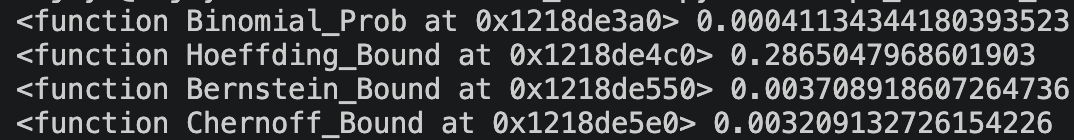
\includegraphics[width=0.9\textwidth]{Section 2.A.png}
    \caption{program outputs in Section 2.A}
    \label{fig:Section2.A}
\end{figure}
From the program outputs, the Chernoff bound is the tightest among these three concentration inequalities, followed by the Bernstein bound. 
The Chernoff and Bernstein bounds are relatively close: they are approximately $7.8$ and $9.02$ times the exact binomial tail probability, respectively.
Thus, both bounds differ from the exact probability by roughly one order of magnitude.

For Hoeffding bound, it is the loosest concentration bound among these three bounds.
It is approximately $696.5$ times the exact binomial tail probability, which is about a three-order-of-magnitude multiplicative gap.
This result matches our expectation that the Hoeffding's inequality is quite loose for small $p$.
Compared with other bounds, it only consider the upper/lower bound of the random variable, instead of considering higher moments (second moment is used for Bernstein bound and moment generating is used for Chernoff bound).

\newpage
\subsection*{Part 2.B}
\begin{figure}[htbp!]
    \centering
    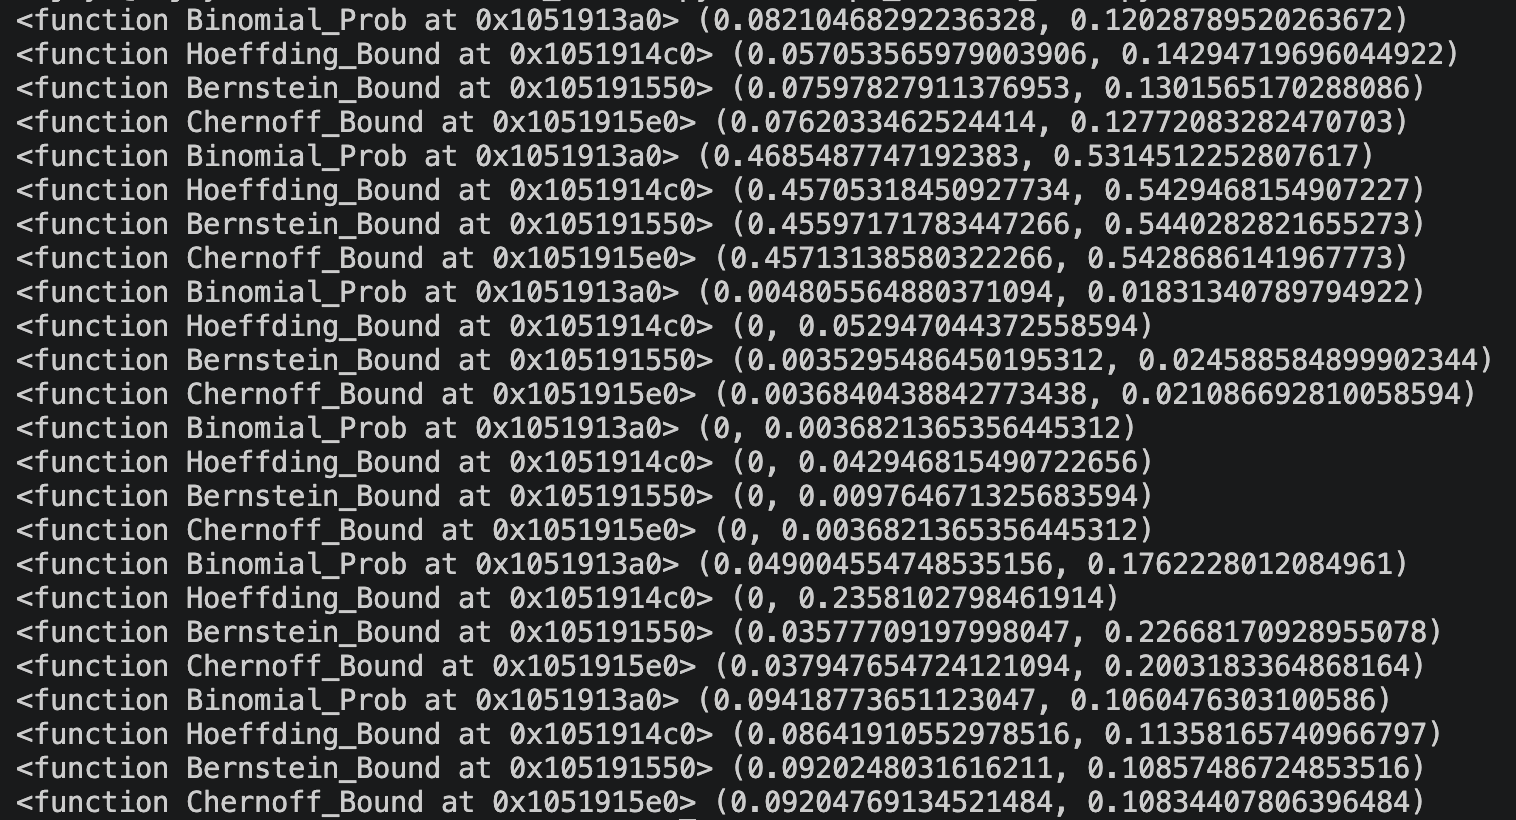
\includegraphics[width=0.9\textwidth]{Section 2.B.png}
    \caption{program outputs in Section 2.B}
    \label{fig:Section2.B}
\end{figure}
\begin{itemize}
    \item [1.] For fixed $k/n$, the confidence interval becomes narrower as $n$ increases. For fixed $n$, the interval is generally wider when $k/n$ is approaching $1/2$.
or \(1\).
    \item [2.] When $k/n$ is small, the confidence interval of the Hoeffding's bound usually has a smaller lower bound and a larger upper bound than other intervals.
    This implies that Hoeffding's inequality is especially looser than the others for small values of $k/n$.
    \item [3.] The ordering observed in Part 2.A is generally reflected in the confidence intervals: a tighter tail bound usually gives a narrower interval.
    This relationship is obvious when $k/n$ is small and there is a distinction between Hoeffding bound and other bounds.
    However, it become vague when $k/n$ is close to $1/2$.
\end{itemize}


\newpage
\subsection*{Part 2.C}
\begin{itemize}
    \item [1.] See the following program outputs.
        \begin{figure}[htbp!]
            \centering
            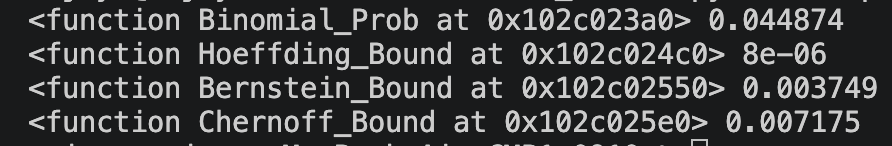
\includegraphics[width=0.9\textwidth]{Section 2.C.png}
            \caption{program outputs in Section 2.C}
            \label{fig:Section2.C}
        \end{figure}
    \item [2.] See the following program outputs with different values for $n,p,\delta$.
        \begin{figure}[htbp!]
            \centering
            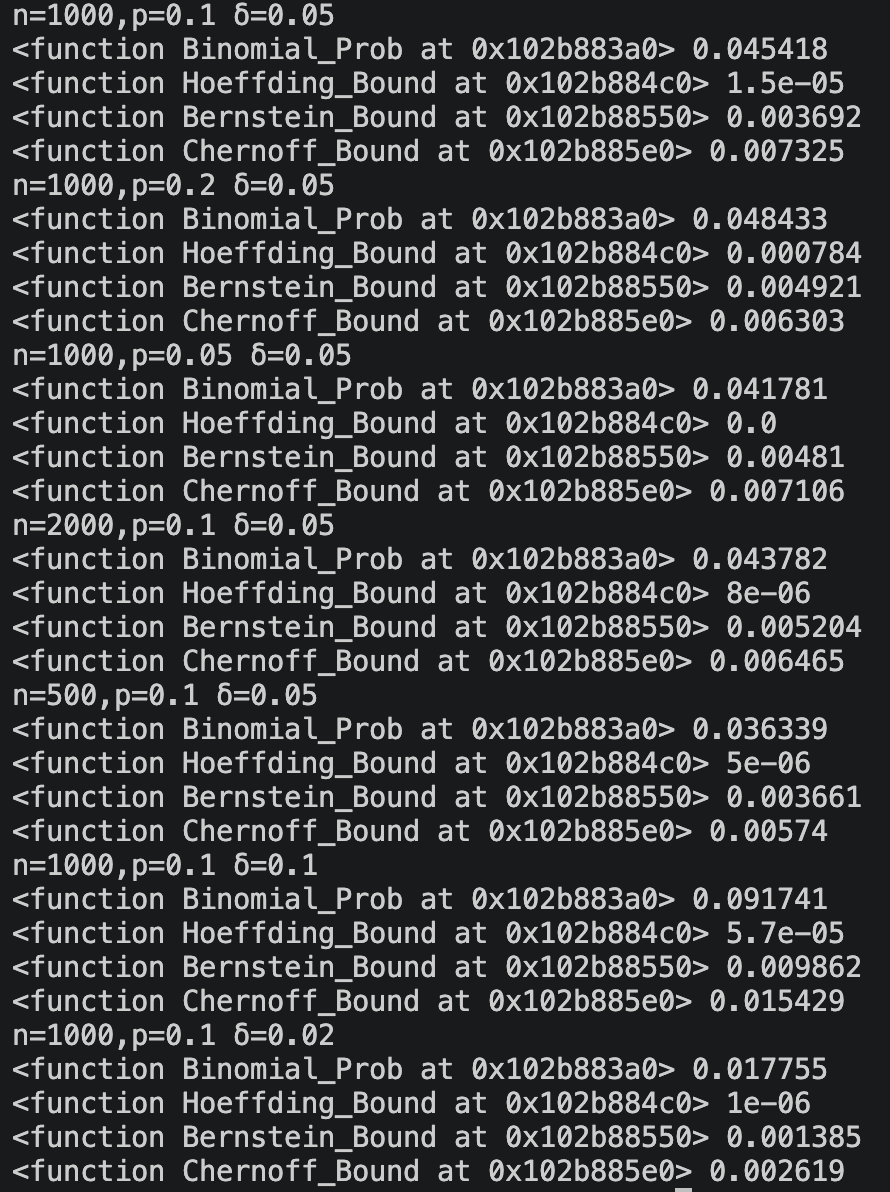
\includegraphics[width=0.6\textwidth]{Section 2.C2.png}
            \caption{program outputs in Section 2.C}
            \label{fig:Section 2.C2}
        \end{figure}
    \item [3.] A tighter bound generally gives a higher miss rate.
    This matches our previous observation. 
    For a loose bound, the corresponding confidence interval is wide.
    Therefore, the true $p$ is less likely to fall outside it, leading to the lower miss rate. 
\end{itemize}

\newpage
\subsection*{Part 2.D}
\begin{figure}[htbp!]
    \centering
    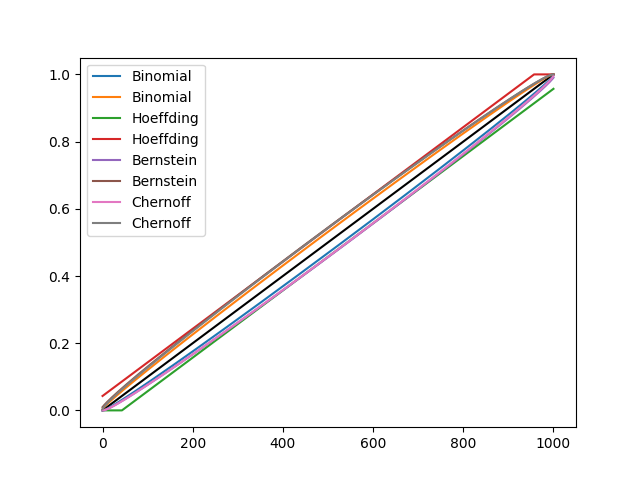
\includegraphics[width=1\textwidth]{plot1.png}
    \caption{$n=1000$, the change of confidence intervals with respect to $k$}
    \label{fig:plot1}
\end{figure}
The first plot shows that the exact binomial interval remains the narrowest, while the Chernoff
interval generally provides the closest approximation to it.
The Chernoff and Bernstein confidence intervals are very close and both approximate the exact binomial interval well.
For Hoeffding bound, it performs similarly as Chernoff and Bernstein when $k$ is far away from both $0$ and $n$ (roughly $k/n$ near $1/2$).
However when $k$ approaches $0$ or $n$, it becomes much looser according to the plot.
This is expected because Hoeffding’s inequality does not exploit the small Bernoulli variance near the boundaries.

The second plot is consistent with these observations.
Since $k/n=0.1$ is relatively small, the Hoeffding interval remains comparatively loose.
The differences are most visible when $n$ is small, where the Chernoff and Bernstein intervals can be clearly distinguished. As $n$ increases, their intervals become increasingly close and contract toward $p=k/n=0.1$.

Near $k/n=1/2$, the Hoeffding, Bernstein, and Chernoff curves almost overlap, so their ordering cannot be clearly distinguished from the plot. However, the numerical results in Part 2.B show that, for \(n=1000\) and \(k=500\), the Bernstein interval is slightly wider than the Hoeffding interval. Thus, the ordering is not uniform across all parameter values.
Besides this, the ordering is almost the same.
\begin{figure}[htbp!]
    \centering
    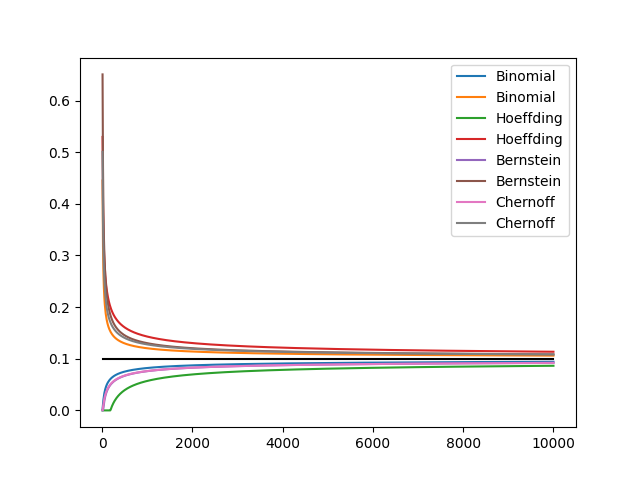
\includegraphics[width=1\textwidth]{plot2.png}
    \caption{$n/k=10$, the change of confidence intervals with respect to $n$}
    \label{fig:plot2}
\end{figure}
\end{document}